%%%%%%%%%%%%%%%%%%%%%%%%%%%%%%%%%%%%%%%%%%%%%%%%%%
\section{Methods}
\label{main:sec:methods}
%%%%%%%%%%%%%%%%%%%%%%%%%%%%%%%%%%%%%%%%%%%%%%%%%%
In this section, we present a novel extension of \gls{npf} called \glspl{mpnp}. The main idea is to elicit joint predictive distributions that are constructed with equivariant neural networks instead of assuming priors for $\theta$, and let the corresponding martingale posterior describe the functional uncertainty in the \glspl{np}. We describe how we construct a \gls{mpnp} in \cref{main:subsec:mpnp} and train it in \cref{main:subsec:training}.

% In \cref{main:subsec:mpnp}, we describe how we construct \gls{mpnp} to generate pseudo context dataset $Z'$ from a given context set $Z_C$. In \cref{main:subsec:training}, we present a training procedure of \gls{mpnp}.

%%%%%%%%%%%%%%%%%%%%%%%%%%%%%%%%%%%%%%%%%%%%%%%%%%
\subsection{Martingale Posterior Neural Processes}\label{main:subsec:mpnp}

Recall that the functional uncertainty in a \gls{np} is encoded in a parameter $\theta$. Rather than learning an approximate posterior $q(\theta|Z_c)$, we introduce a joint predictive $p(Z'|Z_c ; \phi_\text{pred})$ generating a \emph{pseudo context set} $Z' = \{z'_i\}_{i=1}^{N-|c|}$ of size $(N-|c|) \geq 1$. 
% \ed{One question reviewers might ask is why do we use the MP $p(Z' \mid Z_c)$ instead of a more flexible $q(\theta \mid Z_c)$ (e.g. a generative model). Amortization might be a key motivator, which helps us model the deterministic and latent path. It's more natural to combine the pseudo and context data to get $\theta(Z' \cup Z_c)$ than to decode a latent $\theta$ and deterministic $\phi(Z_c)$ through $f(\theta,\phi)$ like in \citep{kim2018attentive}. }
% \ljh{That is actually a good point. One possible answer is that, we can actually go beyond Bayesian inference by using alternative $\ell(z,\theta)$, and say that at least in this work we focused on $\ell$ being negative likelihood to showcase the idea. Another thing we could say is that, we potentially are not sure whether the parameter $\theta$ needs to be finite-dimensional vector; for instance, depending on the application, it would be more natural to assume that $\theta$ itself is a stochastic process. While even the most complex generative models (e.g., normalizing flows) cannot easily deal with them, ours can hypothetically cover that case.
% }
Having generated a pseudo context, we combine with the existing context $Z_c$, and construct the empirical density as
\[
g_N(z) = \frac{1}{N}\bigg(\sum_{i\in c}\delta_{z_i}(z) + \sum_{i=1}^{N-|c|} \delta_{z'_i}(z)\bigg).
\]
Given $g_N$, the estimate of the function parameter $\theta$ is then recovered as 
\[
\label{eq:recovering_theta}
\theta(g_N) := \argmin_\theta \int \ell(z, \theta) g_N(dz),
\]
where in our case we simply choose $\ell(z,\theta) := -\log \calN(y|\mu_\theta(x), \sigma^2_\theta(x)I_\dout)$. The uncertainty in $\theta(g_N)$ is thus induced by the uncertainty in the generated pseudo context $Z'$.

\paragraph{Amortization}
The procedure of recovering $\theta$ via \cref{eq:recovering_theta} would originally require iterative optimization process except for simple cases. Fortunately, in our case, we can \emph{amortize} this procedure, thanks to the mechanism of \glspl{cnp} amortizing the inference procedure of estimating $\theta$ from the context. Given $Z_c$, a \gls{cnp} learns an encoder producing $\theta$ that is trained to maximize the expected likelihood. That is,
\[
 \tilde\theta(Z_c) = f_\text{enc}(Z_c;\phi_\text{enc}), \quad \tilde\theta(Z_c) \approx \argmin_{\theta} \int \ell(z,\theta) g_c(dz),
\]
where $g_c$ is the empirical density of $Z_c$. Hence, given $Z'$ and $Z_c$, we can just input $Z'\cup Z_c$ into $f_\text{enc}$ and use the output $\tilde\theta(Z'\cup Z_c)$ as a proxy for $\theta(g_N)$. Compared to exactly computing $\theta(g_N)$, obtaining $\tilde\theta(Z'\cup Z_c)$ requires a single forward pass through $f_\text{enc}$, which scales much better with $N$. Moreover, computation for multiple $Z'$ required for bagging can easily be parallelized. 

\paragraph{Specifying the joint predictives}
We construct the joint predictives $p(Z'|Z_c;\phi_\text{pred})$ with a neural network. Other than the requirement of $Z'$ being exchangeable (and thus \gls{cid}), we give no inductive bias to $p(Z'|Z_c;\phi_\text{pred})$ and let the model learn $\phi_\text{pred}$ from the data. We thus use the exchangeable generative model described in \cref{main:subsec:exchangeable}. Specifically, to generate $Z'$, we first generate $\calE = \{\varepsilon_i\}_{i=1}^n$ from some distribution (usually chosen to be a unit Gaussian $\calN(0, I_d)$), and pass them through an equivariant \gls{isab} block to form $Z'$. To model the conditioning on $Z_c$, we set the inducing point in the \gls{isab} as a transform of $Z_c$. That is, with an arbitrary feed-forward neural network $h$,
\[
\textsc{isab}(\calE) = \textsc{mab}(\calE, H), \quad H = \textsc{mab}( h(Z_c), \calE ),
\]
where $h(Z_c) = \{h(z_i)\}_{i\in c}$. 
The resulting model is an implicit generative model~\citep{mohamed2016learning} in a sense that we can draw samples from it but cannot evaluate likelihoods.

\paragraph{Generating Representations} 
\begin{figure}[t]
    \centering
    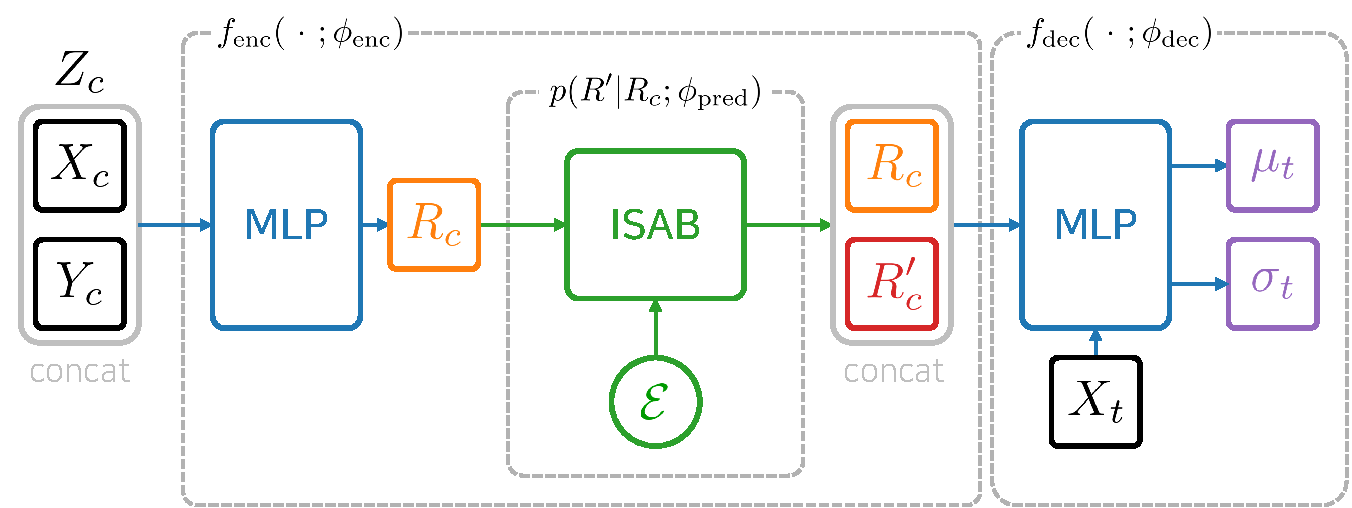
\includegraphics[width=\linewidth]{figure/main_concept.pdf}
    \caption{Concept figure of our feature generating model applied to \gls{cnp}~\citep{garnelo2018conditional}. We first convert given context dataset $Z_c$ to the representation $R_c$ using \gls{mlp} layers. Next we sample $\epsilon$ from a simple distribution (e.g. Gaussian). Then we generate the pseudo context representation $R_c'$ using generator as one layer \gls{isab}~\citep{lee2019set} in our experiment.
    %\ed{This figure is awesome!!}}
    }
    \label{figure/main_concept_mpnp}
\end{figure}
When $z$ is low-dimensional, it would be moderately easy to learn the joint predictives, but in practice, we often encounter problems with high-dimensional $z$, for instance when the input $x$ is a high-resolution image. For such cases, directly generating $z$ may be harder than the original problem, severely deteriorating the overall learning procedure of \gls{mpnp}.
Instead, we propose to generate the \emph{encoded representations} of $z$. The encoders of the most of the \glspl{npf} first encode an input $z_i$ into a representation $r_i$. For the remaining of the forward pass, we only need $r_i$s instead of the original input $z$. Hence we can build a joint predictives $p(R'|R_c; \phi_\text{pred})$ generating $R' = \{r_i'\}_{i=1}^{N-|c|}$ conditioned on $R_c = \{r_i\}_{i\in c}$ as for generating $Z'$ from $Z_c$. In the experiments, we compare these two versions of \glspl{mpnp} (generating $Z'$ and generating $R'$), and found that the one generating $R'$ works much better both in terms of data efficiency in training and predictive performances, even when the dimension of $z$ is not particularly large.
See \cref{figure/main_concept_mpnp} for our method applying to \gls{cnp} model~\citep{garnelo2018conditional}.

%%%%%%%%%%%%%%%%%%%%%%%%%%%%%%%%%%%%%%%%%%%%%%%%%%
\subsection{Training}\label{main:subsec:training}

With the generator $p(Z'|Z_c;\phi_\text{pred})$, the marginal likelihood for a task $\tau = (Z, c)$ is computed as
\[\label{eq:logmarginal_mp}
\log p(Y|X, Z_c) = \log\int \exp\bigg(-\sum_{i\in [n]}\ell(z_i, \tilde\theta(Z_c\cup Z'))\bigg) p(Z'|Z_c;\phi_\text{pred}) \dee Z'.
\]
Note that $p(Z'|Z_c;\phi_{\text{pred}})$ is \gls{cid}, so there exists a corresponding martingale posterior $\pi_N$ such that
\[
\log p(Y|X, Z_c) = \log\int \exp\bigg(-\sum_{i\in [n]}\ell(z_i, \theta)\bigg) \pi_N(\theta|Z_c) \dee \theta.
\]
We approximate the marginal likelihood via a consistent estimator,
\[\label{eq:mpnp_term1}
\log p(Y|X, Z_c) \approx \log \Bigg[ \frac{1}{K} \sum_{k=1}^K \exp\bigg(-\sum_{i\in [n]}\ell(z_i, \tilde\theta(Z_c\cup Z'^{(k)}))\bigg)
\Bigg] := -\calL_\text{marg}(\tau,\phi),
\]
where $Z'^{(1)},\dots, Z'^{(K)}\iidsim p(Z'|Z_c;\phi_\text{pred})$. This objective would be suffice if we are given sufficiently good $\tilde\theta(Z_c \cup Z'^{(k)})$, but we have to also train the encoder to properly amortize the parameter construction process \cref{eq:recovering_theta}. For this, we use only the given context data to optimize
\[\label{eq:mpnp_term2}
\log p_{\textsc{cnp}}(Y|X, Z_c) = -\sum_{i\in [n]} \ell(z_i, \tilde\theta(Z_c)) := -\calL_\text{amort}(\tau,\phi)
\]
that is, we train the parameters $(\phi_\text{enc}, \phi_\text{dec})$ using \gls{cnp} objective. Furthermore, we found that if we just maximize \cref{eq:mpnp_term1} and \cref{eq:mpnp_term2}, the model can cheat by ignoring the generated pseudo contexts and use only the original context to build function estimates. To prevent this, we further maximize the similar \gls{cnp} objectives for each generated pseudo context to encourage the model to actually make use of the generated contexts.
%\ljh{I'm not sure whether this justifies using avg outside the log rather than the avg inside the log.} 
\[\label{eq:mpnp_term3}
\frac{1}{K}\sum_{k=1}^K \log p_{\textsc{cnp}} (Y|X, Z'^{(k)}) = -\frac{1}{K}\sum_{i\in [n]} \ell(z_i, \tilde\theta(Z'^{(k)})) := -\calL_\text{pseudo}(\tau,\phi)
\]
Combining these, the loss function for the \gls{mpnp} is then
\[\label{eq:mpnp_term_whole}
\bbE_{\tau}[\calL(\tau,\phi)] = \bbE_\tau[\calL_\text{marg}(\tau,\phi) + \calL_\text{amort}(\tau,\phi) + \calL_\text{pseudo}(\tau,\phi)].
\]

% \lhg{I submitted our paper to Openreview. You can check that.}
% \ed{Thank you!!}

% \glspl{mpnp} model contains generator function $f_{\gen}$ which generates a pseudo context dataset $Z'$ or a feature of pseudo context dataset $R'$.
% To make a generator of \gls{mpnp} to sample meaningful $Z'$ or $R'$, we need to carefully construct training objective function. Otherwise, the generator tends to sample pseudo context dataset far from context dataset or collapse to one-point which does not have enough meaning or affection to target dataset. We maximize our training objective function which consists of the following terms:
% \begin{align}
%     \sum_{i=1}^n\left(\log p(y_i|x_i,Z_c,\varnothing)+\log \frac{1}{K}\sum_{k=1}^K p(y_i|x_i,Z_c,Z'^{(k)})+\frac{1}{K}\sum_{k=1}^K \log p(y_i|x_i, \varnothing, Z'^{(k)})\right)
% \end{align}
% % \ed{Thanks for updating, much clearer now. Should the third term be $p(y_i \mid x_i, \varnothing, Z'^{(k)})$ then?}
% % \lhg{Yes, that's right. We don't use context data in the third term.}\ed{I added it, hope it's ok!}
% where $K$ is the number of different generated pseudo context dataset.
% Here the first term $\log p(y|x,Z_c, \varnothing)$ implies that our amortized model should also well predict the posterior distribution of $Z$ only with context dataset. 
% The second term implies that the ensemble of our model should well predict the posterior distribution of $Z$ with context dataset and pseudo context dataset.
% The third term implies that our model should generate pseudo context dataset which well explains $Z$.
% This third term makes our model to actually generate more meaningful pseudo context dataset. 
% See \cref{app:sec:ablation_study} for generated pseudo context samples without third loss term.


% \ed{For the third term in (14), would it perhaps make more sense to put the sum inside the log, that is
% $$\log \frac{1}{K} \sum_{k=1}^K p(y_i \mid x_i, \varnothing, Z'^{(k)})$$
% so it is still kind of a posterior predictive density? Will this affect the results much?}\\
% \lhg{We empirical check that $\log \frac{1}{K} \sum_{k=1}^K p(y_i \mid x_i, \varnothing, Z'^{(k)})$ decrease the performances, and defeat by some baselines. And when I tried $\frac{1}{K} \sum_{k=1}^K \log p(y_i \mid x_i, \varnothing, Z'^{(k)})$, somewhat I think was each generated pseudo context set $Z'^{(k)}$ sampled independently and each sample should be sampled meaningfully. I mean if we use $\log \frac{1}{K} \sum_{k=1}^K p(y_i \mid x_i, \varnothing, Z'^{(k)})$, then the generator does not sample each pseudo context dataset meaningfully.}

% \lhg{
% \begin{align}
%     \log \Big(\frac{1}{K}\sum_{k=1}^K \exp{\big(\sum_{i=1}^n \log p(y_i|x_i,Z_c,Z'^{(k)})\big)}\Big) +\sum_{i=1}^n\left(\frac{1}{K}\sum_{k=1}^K \log p(y_i|x_i, \varnothing, Z'^{(k)}) + \log p(y_i|x_i,Z_c,\varnothing)\right)
% \end{align}
% }
% where $K$ is the number of different generated pseudo context dataset. Here, the first term is our posterior predictive density on $Z$, integrating over the posterior distribution of $\theta$ induced by the generator $p(Z_c' \mid Z_c)$.
% The second term  ensures our generator generates meaningful pseudo context dataset which allow the decoder to predict well.  As we are unable to evaluate the marginal likelihood $Z_c$ due to the implicit generative model, we rely on the decoder likelihood to improve the quality of $Z_c'$ samples. \lhg{For this term, we use $\frac{1}{K}\sum_{k=1}^K \log p(y_i|x_i, \varnothing, Z'^{(k)})$ instead of $\log\frac{1}{K}\sum_{k=1}^K  p(y_i|x_i, \varnothing, Z'^{(k)})$ to ensure that our generator samples each $Z'^{(k)}$s independently which well explains $Z$.} See \cref{app:sec:ablation_study} for generated pseudo context samples without this second loss term. The final term $\log p(y|x,Z_c, \varnothing)$ ensures that our amortized model also predicts well with only the context dataset. 

% \ed{Thanks for the explanation on log sum vs sum log - we should add a sentence to justify this. It looks a bit like the first term in the ELBO in equation (7). For the other point, I would prefer to leave in $\varnothing$, since the term $p(y_i \mid x_i,Z_c)$ is ambiguous, as it could be $p(y_i \mid x_i,Z_c, \varnothing)$ or $\int p(y_i \mid x_i,Z_c, Z_c') \, dp(Z_c' \mid Z_c)$. Please correct me if I'm wrong!}

% \lhg{Okay, that will be great. I added some explanations:) I have a Ph.D. admission interview next Tuesday at 16:30 KST so can we keep discussing by e-mail or comments? I understand that martingale posterior distribution is an open problem for model-data mismatch situations, is it correct?}

% \ed{Yes that's no problem, best of luck with the interview! :) @Juho should we cancel the Tuesday meeting then? We can communicate by email. Yep, model misspecification is still an open problem in the martingale posterior framework.}
% \lhg{Okay, great.}
% \ljh{No problem with me either!}

% \ed{The first term in the objective is more like the point-wise log posterior predictive density averaged over the $n$ data points, which is the KL divergence between the empirical distribution of $\mathcal{D}$ and the posterior predictive $p(y \mid x,Z_c)$.}

% \lhg{We changed our objective function. The first term changed from $\sum_{i=1}^n \log \frac{1}{K}\sum_{k=1}^K p(y_i|x_i,Z_c,Z'^{(k)})$ to $\log \Big(\frac{1}{K}\sum_{k=1}^K \exp{\big(\sum_{i=1}^n \log p(y_i|x_i,Z_c,Z'^{(k)})\big)}\Big)$.}

% \ed{
% % Nice!! And this work well? The objective is looking much better motivated now :) 
% % For the third term, we previously tried putting the avg inside the log, that is
% % $$\sum_{i \in [n]} \log \frac{1}{K} \sum_{k =1}^K  \exp\left(-\ell(z_i, \tilde\theta(Z'^{(k)}))\right),$$ and it didn't work well right? 
% Following the recent change to $\mathcal{L}_{\text{marg}}$, what about 
% $$
%  -\mathcal{L}_{\text{pseudo}}^*(\phi) =  \log \frac{1}{K} \sum_{k =1}^K  \exp\left(-\sum_{i \in [n]} \ell(z_i, \tilde\theta(Z'^{(k)}))\right),
% $$
% which is basically the first term, so a marginal likelihood, but only using $Z'^{(k)}$. The current $-\mathcal{L}_{\text{pseudo}}$ is a just lower bound on $-\mathcal{L}_{\text{pseudo}}^*$ from Jensen's inequality. 
% %Because of this, I'm guessing the results will be similar. 
% The objective would be nice and symmetric now, since it's essentially 3 (marginal) likelihood terms, corresponding to context + pseudo, only context and only pseudo.
% % If we're short on time, we can motivate $-\mathcal{L}_{\text{pseudo}}$ as being a lower bound to $-\mathcal{L}^*_{\text{pseudo}}$, that is perhaps numerically more stable. Really sorry for giving you more work Hyungi!!
% }
% \lhg{Actually, we simultaneously tried that term in experiment with (18) and sadly it didn't work well...So we fixed (18). Maybe we can justify with lower bound or something else.}
% \ed{Ah damn, that's unfortunate. Maybe we can stick to the lower bound justification then and point to the Supplementary.}
% \lhg{Yep, that will be good. Now we are trying $\lambda\calL^*$ with additional scaling factor $\lambda\geq 1$.}
% \ed{That's a good idea, perhaps we need to balance $\mathcal{L}_{\text{pseudo}}$ with $\mathcal{L}_{\text{amort}}$?}
% \lhg{That's a good point.}
% \paragraph{Main approach}
% \glspl{np} are interested in learning a latent function $f$ such that
% \begin{align*}
%     f\sim p(f),\quad y|x,f\sim p(y|x,f)
% \end{align*}
% where $(x,y)\in \calD$.
% For instance, $f$ may be parameterized by decoder neural networks of \glspl{np}, $\mu_{\dec}(\cdot;\theta)$ and $\sigma_{\dec}(\cdot;\theta)$, such that
% \begin{align*}
%     \theta\sim p(\theta),\quad y|x,\theta\sim \calN(y|\mu_{\dec}(x;\theta),\sigma_\dec^2 (x;\theta)).
% \end{align*}
% In martingale posterior neural processes, instead of assuming a prior (either for $p(f)$ or $p(\theta)$), we directly model a conditional joint predictive distributions of pseudo context dataset as,
% \begin{align*}
%     \calD_{C'}\sim p_\phi (\calD_{C'}|\calD_C),
% \end{align*}
% where $\phi$ is a parameter of joint predictive distribution and $\calD_{C'}=\{(x_i',y_i')\}_{i=1}^{n_g}$ is a generated pseudo context dataset with number of generated pseudo context data $n_g\geq 1$.
% If $(x,y)$ is high-dimensional (such as images), we can instead consider an encoded vector $r_C=f_{\enc}(\calD_C)$ and learn the joint predictive distribution of the encoded representations as $p_\phi (r_{C'}|r_C)$. Using this predictive, we can construct an empirical predictive density as
% \begin{align*}
%     g_N(x,y) = \frac{1}{|c|+n_g}\left(\sum_{i\in c}\delta_{(x_i,y_i)} + \sum_{i=1}^{n_g}\delta_{(x_i',y_i')}\right).
% \end{align*}
% The estimate of the function parameter $\theta$ should originally be obtained as
% \begin{align*}
%     \theta(g_N):=\argmin_\theta\int \ell((x,y),\theta)g_N(dx,dy),
% \end{align*}
% where in our case we set
% \begin{align*}
%     \ell((x,y),\theta)=-\log \calN (y|\mu_{\dec}(x;\theta),\sigma_{\dec}^2(x;\theta)).
% \end{align*}
% Instead of directly solving this, we introduce an amortization network with parameter $\lambda$ such that
% \begin{align*}
%     \hat{\theta}(\calD_C\cup\calD_{C'};\lambda)\approx \theta(g_N).
% \end{align*}
% Here we can see that differently generated pseudo context dataset $\calD_{C'}^{(1)}=\{(x_i'^{(1)},y_i'^{(1)})\}_{i=1}^{n_g}$ and $\calD_{C'}^{(2)}=\{(x_i'^{(2)},y_i'^{(2)})\}_{i=1}^{n_g}$ formulate different empirical predictive densities.
% Different predictive densities also formulate different amortized $\hat{\theta}$ which models functional uncertainty without both a global latent variable and a custom prior distribution.
% If we have chosen to learn the predictive of encoded representations, we first have to learn $\hat{\theta}(\cdot;\lambda)$ using only real context representation $r_C$, and put generated representation $r_{C'}$ into the amortization network later.
% \paragraph{Directly generating pseudo context data}
% In order to construct an empirical predictive density $g_N(x,y)$, we have to sample a pseudo context dataset. 
% The most straightforward approach to generate pseudo context dataset $\calD_{C'}$ is directly generating $(x_i',y_i')$ from given context dataset $\calD_C$.
% Our first attempt to formulate generator function $f_{\gen}$ was to na\"ively use ISAB~\citep{lee2019set} module as our generator and sample whole $D_{C'}$ at once.
% We use concatenated $D_C$ as inducing points $I\in\bbR^{|C|\times 2}$ in ISAB and $g$, which is \textit{i.i.d} samples from Gaussian distribution, as input $\bx\in \bbR^{n_g\times 2}$.
% Because ISAB module satisfies permutation invariance for input dataset, we can directly sample a set $\calD_{C'}$ without break exchangeability...
% \paragraph{Generating features of pseudo context data}
% \begin{figure}[t]
%     \centering
%     \includegraphics[width = \linewidth]{figure/feature model2.pdf}
%     \caption{Concept figure of our feature generating model applied to \gls{canp}~\citep{kim2018attentive}. Here we sample $g$ from a simple distribution (e.g. Gaussian). We generate key feature $r_k'$ and value feature $r_v'$ for cross attention layer which are corresponding to pseudo context data. We use generator as one layer ISAB~\citep{lee2019set} in our experiment.}
%     \label{fig:feature model2.pdf}
% \end{figure}
% As we mentioned above paragraph, directly generating pseudo context dataset is hard task, we construct our model to sample features of pseudo context dataset.
% We first encode our $\calD_c$ into $r_c\in\bbR^{|C|\times r_\text{dim}}$ with our encoder neural network $f_{\enc}$.

% See \cref{fig:feature model2.pdf} for our method applying to \gls{canp} model~\citep{kim2018attentive}.
% \subsection{Training}
% \label{main:subsec:training}
% \glspl{mpnp} model contains generator function $f_{\gen}$ which generates a pseudo context dataset $\calD_{C'}$ or a feature of pseudo context dataset $r_{C'}$.
% To make a generator of \gls{mpnp} to sample meaningful $\calD_{C'}$ or $r_{C'}$, we need to carefully construct training objective function. Otherwise, the generator tends to sample pseudo context dataset far from context dataset or collapse to one-point which does not have enough meaning or affection to target dataset. We consist our training objective function as maximizing following terms:
% \begin{align}
%     \sum_{i=1}^n\left(\log p(y_i|x_i,\calD_C)+\log \frac{1}{K}\sum_{j=1}^K p(y_i|x_i,\calD_C,\calD_{C'}^{(j)})+\frac{1}{K}\sum_{j=1}^K \log p(y_i|x_i, \calD_{C'}^{(j)})\right)
% \end{align}
% \ed{Does the $p$ in the first term above need a subscript? So something like $p_{\text{amort}}$ or something?}

% where $K$ is the number of different generated pseudo context dataset.
% Here the first term $\log p(y|x,\calD_C)$ implies that our amortized model should also well predict the posterior distribution of $\calD$ only with context dataset. 
% The second term implies that the ensemble of our model should well predict the posterior distribution of $\calD$ with context dataset and pseudo context dataset.
% The third term implies that our model should generate pseudo context dataset which well explains $\calD$.
% This third term makes our model to actually generate more meaningful pseudo context dataset. 
% See \cref{app:sec:ablation_study} for generated pseudo context samples with and without each loss terms.
